\documentclass[twocolumn,oneside,12pt,a4paper]{article}

% Import packages
\usepackage{mathtools,amssymb,amsmath,booktabs, graphicx, tabularray, caption, stackengine, multirow} % imports amsmath
\usepackage[T1]{fontenc}

\begin{document}

\title{Using Tesseract OCR to assist KG pupils to learn writing}
\author{Ephrim Lawrence}
\date{}

\twocolumn[
\begin{@twocolumnfalse}
  \maketitle

    % Abstract
  \begin{abstract}
    The paper explores the use of Optical Character Recognition (OCR) technology to assist kindergarten pupils in learning how to write English characters. OCR is a technology that allows computers to recognize printed or handwritten characters and convert them into machine-encoded text, allowing it to be analyzed by a computer. The software presented in this paper provides a platform for pupils to practice writing English alphabets on a computer device, and the OCR technology recognizes and evaluates the accuracy of the pupils' writing. The software also gives immediate feedback to the pupils, enabling them to identify and correct errors in their writing.
  \end{abstract}
\end{@twocolumnfalse}
]

\section{Introduction}
\paragraph*{}
Handwriting is a fundamental skill for literacy development, particularly in the early years of education. For young learners, developing legible and fluent handwriting skills is a critical component of academic success \cite{berninger_writing_2002,dinehart_associations_2013,longcamp_influence_2005,longcamp_remembering_2006}. However, teaching young children to write can be challenging, particularly for pupils with different learning abilities. In recent years, there has been growing interest in the use of technology to support early literacy development, including the use of Optical Character Recognition (OCR) technology to assist pupils in learning how to write English characters. OCR technology has been used in a variety of applications, including document scanning and digitization, automated data entry, and language translation. In the context of literacy education, OCR technology has been used to evaluate and provide feedback on handwriting skills.

For example, a study by \cite{alvaro_basic_2010} conducted with professional school teachers and parents revealed that the handwriting learning software (developed by the authors) for children, which uses a stylus on a touch screen monitor, is appropriate for children's comprehension level and provides a user-friendly, functional, reliable, and correct alternative way of teaching basic handwriting.

While previous studies have demonstrated the potential benefits of OCR technology and other software programs in supporting early literacy development, there is a need for further research to explore efficient OCR algorithms for supporting the development of handwriting skills in young learners. Therefore, this study aims to develop software that uses the Tesseract OCR engine \cite{smith_overview_2007} to assist kindergarten pupils in learning how to write English characters.

The paper is organized into three (4) main sections; Section 1 is the introduction; Section 2 discusses related works on the topic; Section 3 discusses how the systems works and its various components; Section 4 ends the paper by discussing some limitations in the proposed system as well as what can be improved in future works on the topic.

\section{Related Works}
\paragraph*{}
Handwriting is a fundamental skill for literacy development, particularly in the early years of education. For young learners, developing legible and fluent handwriting skills is a critical component of academic success. However, teaching young children to write can be challenging, particularly for pupils with different learning abilities. In recent years, there has been growing interest in the use of technology to support early literacy development, including the use of Optical Character Recognition (OCR) technology to assist pupils in learning how to write English characters.

\cite{alvaro_basic_2010} conducted a study with professional school teachers and parents revealed that the handwriting learning software for children, which uses a stylus on a touch screen monitor, is appropriate for children's comprehension level and provides a user-friendly, functional, reliable, and correct alternative way of teaching basic handwriting.

In \cite{tang_web-based_2006} study, the authors presented a web-based Chinese handwriting education system that provides automatic feedback and analysis to assist students in learning how to write Chinese characters. The system uses handwriting recognition and machine learning techniques to evaluate students' handwriting and provide immediate feedback on the accuracy and fluency of their writing. The study found that the system was effective in improving students' handwriting skills and increasing their motivation and engagement in the learning process.

\cite{longcamp_remembering_2006} compares the effects of handwriting and typing on letter recognition. The study found that handwriting leads to better recognition of letter orientation than typing, especially after some time has passed since learning. The study suggests that the motor activity involved in handwriting helps to form more stable letter representations in memory.

A study by \cite{zin_handwritten_2021} proposed an offline self-learning application to help primary-level students in developing countries learn written English and basic calculations. Handwritten characters or words written on tablets were saved as input images, and a proposed character segmentation method is used to recognize segmented characters with the help of a Convolutional Neural Network (CNN). Handwritten data was collected from primary-level students to build the dataset. The proposed system achieved 95.6\% accuracy on 1000 randomly selected words and 98.7\% for each character, making it a promising solution for improving access to quality education in developing countries.

These studies demonstrate the feasibility and effectiveness of using OCR to assist young people to learn how to write. However, there are still some challenges and limitations that need to be addressed. For example, OCR accuracy may vary depending on the quality of the images, the complexity of the characters, and the diversity of the handwriting styles \cite{asad_high_2016,faizullah_survey_2023,ye_document_2013}. OCR feedback may also not be sufficient or appropriate for all learners, as different children may have different needs and preferences.

\section{Proposed System}
\paragraph*{}
The proposed system is a web-based application that enables pupils to learn the writing of English alphabets. The system uses Tesseract \cite{smith_overview_2007} as the Optical Character Recognition (OCR) engine as well as the HTML Canvas API for the drawing functionality.

When the user opens the app, randomly generated English alphabets are presented to the user. After drawing the alphabet, the user then clicks on the \textit{Check Answer} button to get feedback on whether what was drawn is correct or not. If it matches the generated alphabet, congratulations confetti is shown (this makes the application fun to use), else failure confetti is shown to the user. Figure \ref{fig:start_state} shows the state of the web app on the first start. Figure \ref{fig:success_confetti} shows the state of the app if the alphabet written by the user matches the generated alphabet whilst Figure \ref{fig:failure_confetti} shows the state of the app if the written alphabet is different from the generated one. \\
Figure \ref{fig:app_flowchat} shows the flowchart of the application.


\begin{figure}
  \centering
  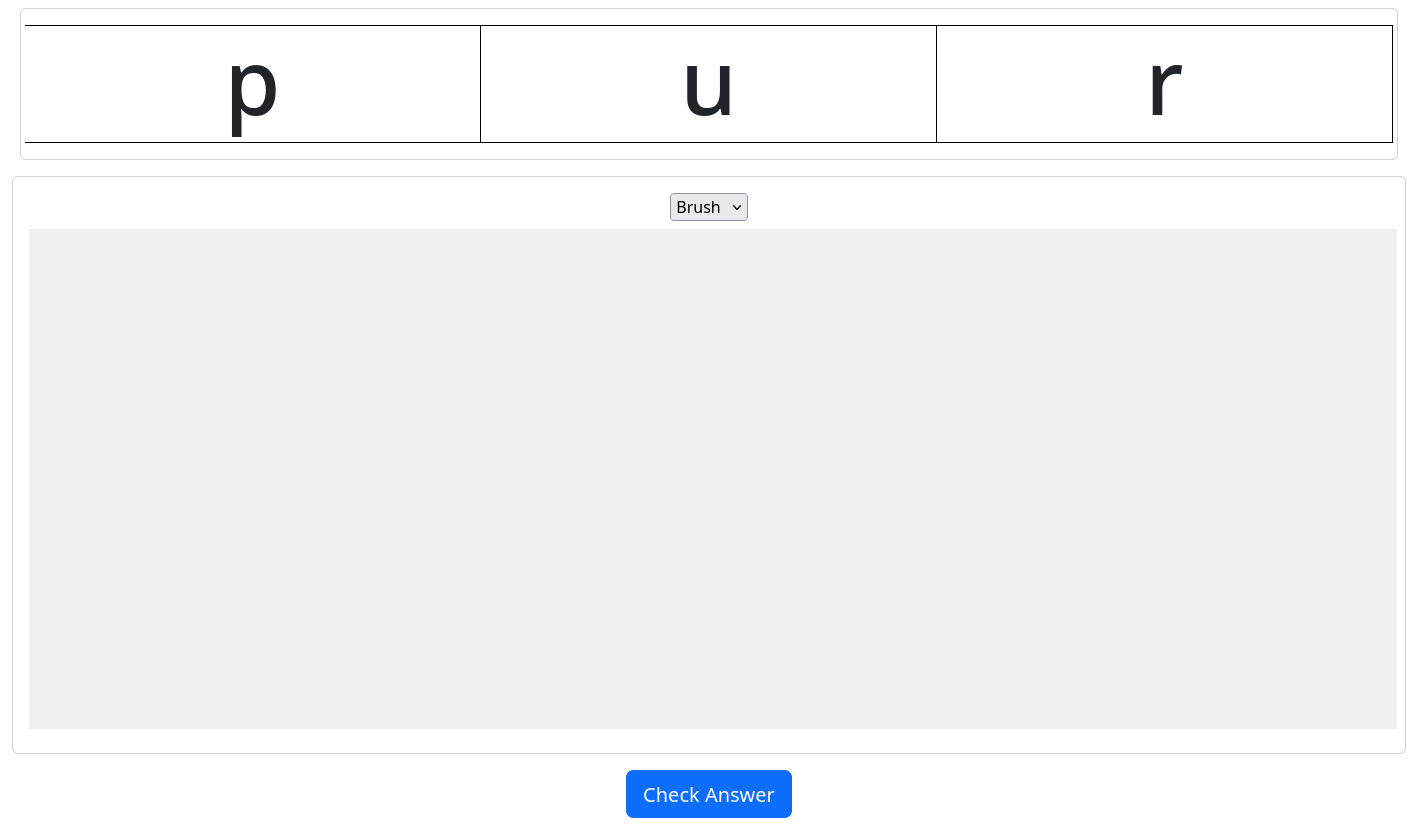
\includegraphics[width=\linewidth]{../start_state.png}
  \caption{UI of the app when it is opened}
  \label{fig:start_state}
\end{figure}

\begin{figure}
    \centering
    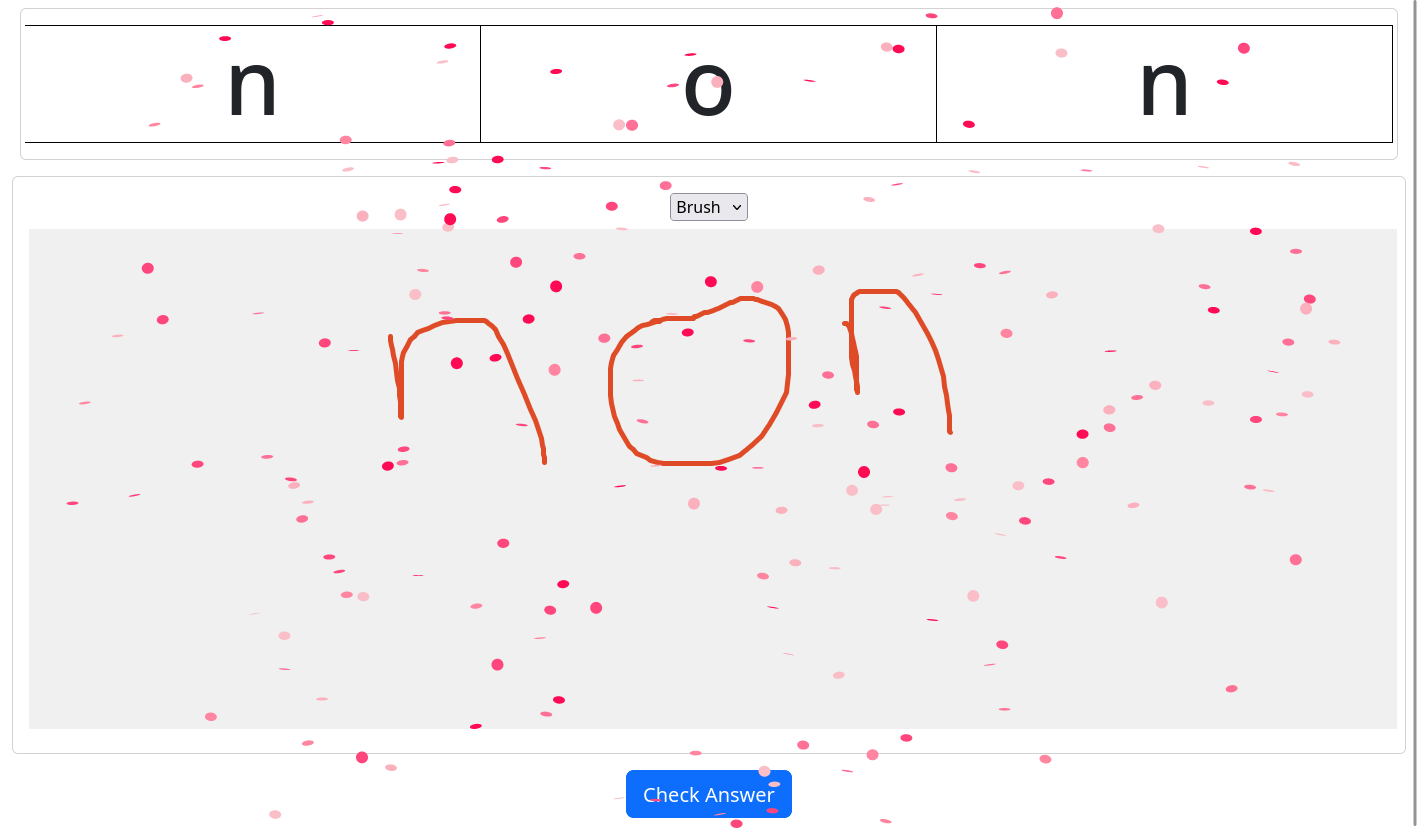
\includegraphics[width=\linewidth]{../success.png}
    \caption{Success confetti when the written alphabets is correct}
    \label{fig:success_confetti}
\end{figure}

\begin{figure}
    \centering
    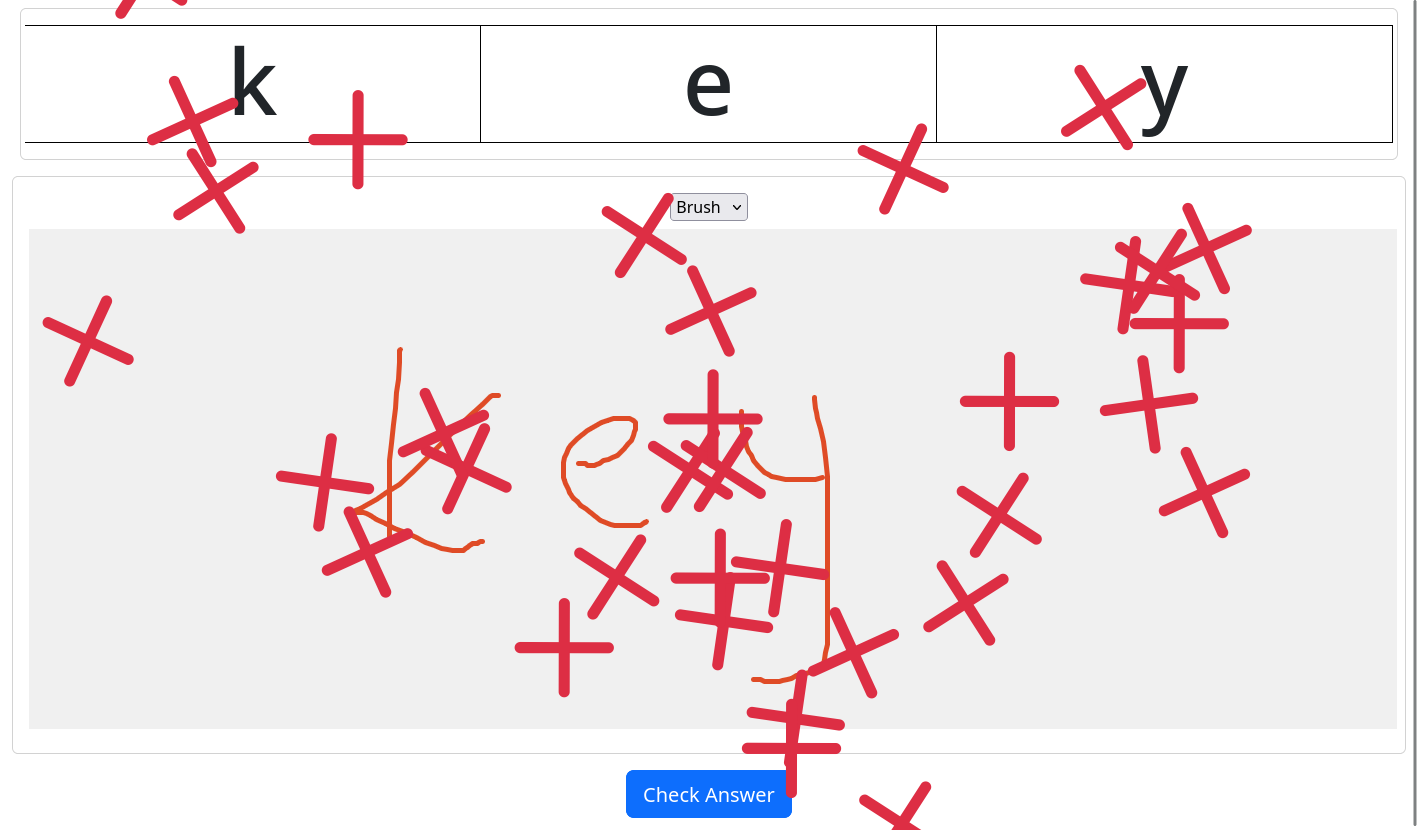
\includegraphics[width=\linewidth]{../failure.png}
    \caption{Failure confetti when the written alphabets is wrong}
    \label{fig:failure_confetti}
\end{figure}

\begin{figure}
    \centering
    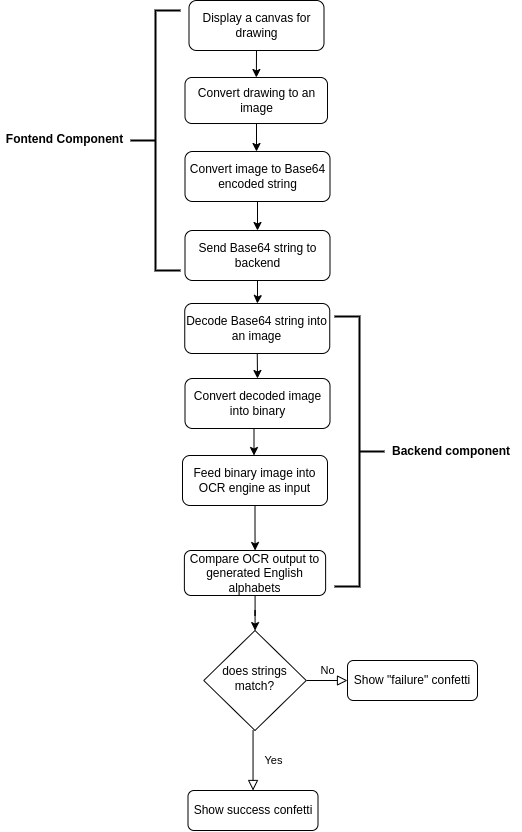
\includegraphics[width=\linewidth]{../flowchat.png}
    \caption{Flowchart of the web application}
    \label{fig:app_flowchat}
\end{figure}

\subsection{Architecture}
\paragraph*{}
The proposed system is divided into three (3) main components; Front-end, Backend and the OCR component. The front end communicates with the backend component via a RESTful API. When the user clicks on the \textit{Check Answer} button, the drawing is converted to an image and then encoded as a Base64 string. The Base64 string is sent via the RESTful API to the backend server. The server decodes the Base64 string back to an actual image and converts the resulting image into a binary image. The binary image is then fed into the Tesseract OCR Engine. The resulting output from the OCR engine is submitted back to the frontend component. On the frontend, the OCR output is compared to the original alphabet, if both strings match success confetti is shown to the user otherwise a failure confetti is displayed to the user. Figure \ref{fig:system_architecture} shows the architecture of the proposed system.

\begin{figure}
    \centering
    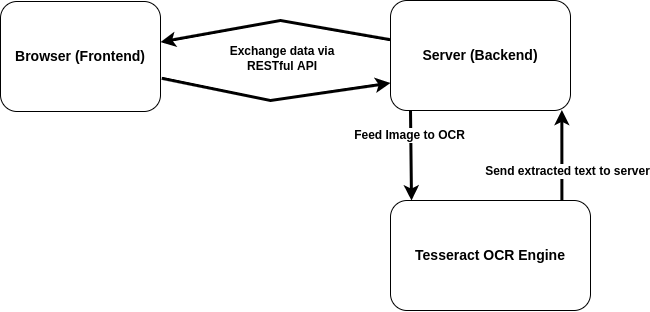
\includegraphics[width=\linewidth]{../system-component.png}
    \caption{Architecture of the web application}
    \label{fig:system_architecture}
\end{figure}

\subsection{Frontend Component}
\paragraph*{}
The frontend component was built with ReactJS \cite{noauthor_react_2023}. ReactJS is a popular open-source JavaScript library used for building user interfaces for web applications; it allows developers to create reusable User Interface (UI) components and efficiently manage the state of the UI. The application uses KonvaJS \cite{noauthor_konvajs_2023} plugin for the drawing functionality. KonvaJS is a 2D graphics library for JavaScript that enables developers to create and manipulate graphical elements on an HTML5 canvas. It provides an easy-to-use API and supports various features such as drag and drop, animations, and event handling.

\subsection{Backend Component}
\paragraph*{}
The backend server was built using Python programming language and FastAPI web framework. FastAPI is a modern, fast, and type-safe web framework for building APIs with Python 3.9+ based on the open standards for APIs (OpenAPI); it provides a simple, intuitive, and high-performance interface for building APIs with minimal boilerplate code.

\subsection{Image Processing}
\paragraph*{}
The image is sent as a Base64 encoded string to the server via RESTful API. The server decodes the string into an actual image. The colour image is converted into a binary image using Otsu’s thresholding algorithm \cite{bangare_reviewing_2015}. The resulting binary image is then fed into Tesseract OCR to identify the characters in the image. The output is compared to the original alphabet to check for accuracy. Figure \ref*{fig:image_processing_pipeline} shows graphical representation of the image processing pipeline used in this paper.

\begin{figure}
    \centering
    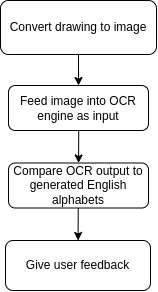
\includegraphics[]{../image-pipeline.png}
    \caption{Image processing pipeline}
    \label{fig:image_processing_pipeline}
\end{figure}

\section{Limitation}
\paragraph*{}
It was discovered in the testing phase of the application that the accuracy of the Tesseract OCR engine is poor when using an image which has few characters. This is because Tesseract OCR relies heavily on contextual information to recognise characters correctly. In the case of single-character images, little or no contextual information is available, which can lead to errors.
Tesseract OCR uses machine learning algorithms to recognize characters, and the accuracy of the OCR can depend on the quality and quantity of the training data available. If the training data does not include enough examples of single-character images, the OCR accuracy may be lower. Unlike \cite{zin_handwritten_2021}, this study did not collect any handwritten dataset to retrain the Tesseract OCR neural network. This, therefore, resulted in low accuracy when recognising handwritten text.
However, there are methods to improve the accuracy of the Tesseract OCR engine as mentioned in \cite{hengaju_improving_2023,sporici_improving_2020}.

\section{Conclusion}
\paragraph*{}
The paper explored how to leverage the Tesseract OCR engine to assist KG pupils in learning the writing of the English alphabet. A web application that allows pupils to learn writing was presented in this paper. The application randomly generates a set of English alphabets. Users (KG pupils) then draw the alphabets and Tesseract OCR is used to check if the alphabets were written correctly.

\section{Future Works}
\paragraph*{}
Future studies on leveraging OCR to assist young people in learning writing can implement or (using existing OCR) which extracts text images with few or even single characters. Text to Speech (in the native language of the learner) functionality can also be added to make the learning process more interactive and fun. The Text-to-Speech functionality can spell out the alphabet to write and also give step-by-step instructions on how to write the alphabet.

\clearpage
\bibliographystyle{apalike}
\bibliography{bibliography.bib}

\end{document}
